\documentclass{article}
\author{Tyler Compton}
\title{Section 10.2 - Vectors}

\usepackage{graphicx}
\usepackage{float}
\usepackage{amsfonts}
\usepackage{gensymb}
\usepackage{amsmath}
\usepackage{esvect}
\graphicspath{ {images/} }

\begin{document}

\maketitle
\tableofcontents

\section{Introduction}
Vectors are geometric elements that represent a direction and magnitude. An
example of a vector is velocity. When we say a car is going 45 miles per hour
in the north-west direction, we've constructed a vector that represents the
car's movement.

\section{Vector Naming and Representation}
Vectors are represented by an arrow on a graph.

\begin{figure}[H]
	\centering
	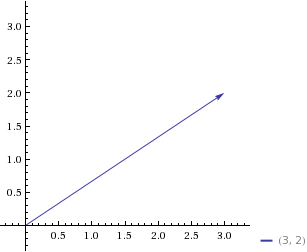
\includegraphics[width=8cm]{vector}
	\caption{An example of a vector in $\mathbb{R}^2$}
	\label{fig:vector}
\end{figure}

The above vector starts at the origin (0, 0), and extends to the point (3, 2).
The point where the vector starts is known as the vector's ``tail''. The point
it ends at is referred to as its ``head''.

If we decided to name the point (0, 0) A and point (3, 2) the name B, we could
refer to the instance of this vector as $\vv{AB}$. When we use this notation,
we are referring specifically to the vector at this position. A vector at some
other position with the same direction and magnitude cannot be referred to as
$\vv{AB}$

We could also refer to \ref{fig:vector} with a letter, like $\vv{\nu}$. Since
our new name makes no mention of the points the vector is on, the only
qualification we're worried about is the vector itself. Vectors don't
inherently contain position information, so our vector $\vv{\nu}$ could be put
anywhere.

\section{Creating Vectors}
As mentioned earlier, vectors have two components: magnitude and direction. In
the car example in the introduction, the magnitude would be the speed of the
car and the direction would be the way the car is pointing.

We oftentimes create vectors by using the format $<3, 2>$, where 3 is the
distance the vector travels in the x direction and 2 is the distance it travels
in the y direction. Because we're representing the vector direction in terms of
distance, the magnitude can be derived from these values easily through
trigonometry and therefore does not have to be explicitly supplied. Remember
that these values are directional, so if you want to construct a vector that
goes down and to the left, it would be $<-3, -2>$.

\section{Arithmatic Operations on Vectors}

\subsection{Addition}
Vector addition is done in a way similar to how matrix addition is done.
Elements of the same type are added together.

$$<3, 4> + <2, 1> = <5, 5>$$

Vectors are added from head to tail. There's no good way to describe what that
means, but as usual, a picture is worth a thousand words.

\begin{figure}[H]
	\centering
	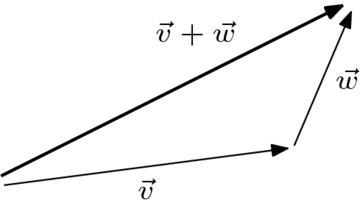
\includegraphics[width=8cm]{vector-addition}
	\caption{Two vectors being added together from head to tail.}
	\label{fig:vector-addition}
\end{figure}

\subsection{Subtraction}
Subtraction works in exactly the same way as addition.

$$<3, 4> - <2, 1> = <1, 3>$$A

\begin{figure}[H]
	\centering
	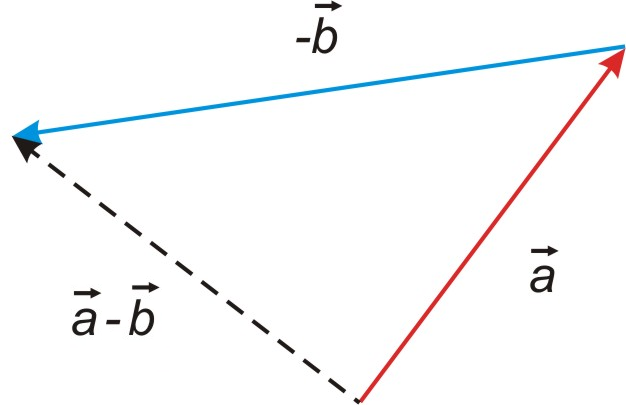
\includegraphics[width=8cm]{vector-subtraction}
	\caption{Vector subtraction is done from head to tail, as well.}
	\label{fig:vector-subtraction}
\end{figure}

\subsection{Multiplying Scalars Onto Vectors}
You can multiply a scalar quantity (commonly known as a regular number) onto a
vector. It does what you might expect. The scalar is distributed onto each
component of the vector.

$$(3)<2, 4> = <6, 12>$$

The effects on the vector's magnitude are intuitive. Below is a graph of a
vector and another graph of the same vector multiplied by two.

\end{document}
